%%%%%%%%%%%%%%%%%%%%%%%%%%%%%%%%%%%%%%%%%%%%%%%%%%%%%%%%%%%%%%%%%%%%%%%%
%                                                                      %
% LaTeX, FIIW thesis template                                          %
%                                                                      %
%%%%%%%%%%%%%%%%%%%%%%%%%%%%%%%%%%%%%%%%%%%%%%%%%%%%%%%%%%%%%%%%%%%%%%%%
\documentclass[11pt,a4paper]{report}
% Indien je je thesis recto-verso wil afdrukken gebruik je onderstaande opties i.p.v. bovenstaande
%\documentclass[11pt,a4paper,twoside,openright]{report}

\usepackage[a4paper,left=3.5cm, right=2.5cm, top=3.5cm, bottom=3.5cm]{geometry}
\usepackage[english]{babel}
\usepackage{graphicx}
\usepackage[latin1]{inputenc}           % om niet ascii karakters rechtstreeks te kunnen inputten
%\usepackage[utf8]{inputenc}            % commentarieer deze regel uit als je utf8 encoded files gebruikt in plaats van latin1
\usepackage{natbib}
\usepackage{listings}             		% voor het weergeven van broncode
\usepackage{verbatim}					% weergeven van code, commando's, ...
\usepackage{hyperref}					% maak PDF van de thesis navigeerbaar
\usepackage{url}						% URL's invoegen in tekst met behulp van \url{http://}
\usepackage[small,bf,hang]{caption}     % om de captions wat te verbeteren
\usepackage[final]{pdfpages}            % gebruikt voor het invoegen van het artikel in pdf-formaat
\usepackage{pslatex}					% andere lettertype's dan de standaard types
\usepackage{lipsum}
\usepackage{sectsty}					% aanpassen van de fonts van sections en chapters
%\usepackage[nottoc,numbib]{tocbibind}	% Bibliography mee in de ToC
\usepackage{fancyvrb,newverbs,xcolor}

\allsectionsfont{\sffamily}
\chapterfont{\raggedleft\sffamily}

\usepackage{float}                      % De optie H voor de plaatsing van figuren op de plaats waar je ze invoegt. bvb. \begin{figure}[H]
%\usepackage{longtable}					% tabellen die over meerdere pagina's gespreid worden
%\usepackage[times]{quotchap}           % indien je fancy hoofdstuktitels wil
%\usepackage[none]{hyphenat}
%\usepackage{latexsym}
%\usepackage{amsmath}
%\usepackage{amssymb}
\usepackage{wrapfig}					% figuren met text die er rond wrapt
\usepackage{minibox}					% voor randen rond multilijn text

% MFA: zet zoekpad voor figure
\graphicspath{{fig/}}

\usepackage{fiiw}
%\usepackage{fiiw_eng} % For the english version (also change last page at the bottom of this file!

%%%%%%%%%%%%%%%%%%%%%%%%%%%%%%%%%%%%%%%%%%%%%%%%%%%%%%%%%%%%%%%%%%%%%%%%%%%%%%%%%%%%%%%%
% OWN ADDED CODE

%for the grey background in codeblocks
\definecolor{cverbbg}{gray}{0.93}        % <== COLOR FOR THE CODE BOX IN LCVERB
\newenvironment{cverbatim}
{\SaveVerbatim{cverb}}
{\endSaveVerbatim
	\flushleft\fboxrule=0pt\fboxsep=.5em
	\colorbox{cverbbg}{\BUseVerbatim{cverb}}%
	\endflushleft
}
\newenvironment{lcverbatim}
{\SaveVerbatim{cverb}}
{\endSaveVerbatim
	\flushleft\fboxrule=0pt\fboxsep=.5em
	\colorbox{cverbbg}{%
		\makebox[\dimexpr\linewidth-2\fboxsep][l]{\BUseVerbatim{cverb}}%
	}
	\endflushleft
}
\newcommand{\ctexttt}[1]{\colorbox{cverbbg}{\texttt{#1}}}
\newverbcommand{\cverb}
{\setbox\verbbox\hbox\bgroup}
{\egroup\colorbox{cverbbg}{\box\verbbox}}


%%%%%%%%%%%%%%%%%%%%%%%%%%%%%%%%%%%%%%%%%%%%%%%%%%%%%%%%%%%%%%%%%%%%%%%%%%%%%%%%%%%%%%%%



%door onderstaande regels in commentaar te zetten, of op false, kan je pagina's weglaten
%bijvoorbeeld het weglaten van een voorwoord, lijst met symbolen, ...
%%%%%%%%%%%%%%%%%%%%%%%%%%%%%%%%%%%%%%%%%%%%%%%%%%%%%%%%%%%%%%%%%%%%%%%%%%%%%%%%%%%%%%%%
%voorwoord toevoegen?
\acknowledgementspagetrue
\acknowledgements{voorwoord}			%.tex file met daarin het voorwoord

%samenvatting toevoegen
\summarypagetrue
\summary{samenvatting}					%.tex met daarin de samenvatting

%abstract toevoegen?
\abstractpagetrue
\abstracts{abstract}					%.tex file met daarin het abstract
%lijst van figuren toevoegen?
\listoffigurespagetrue
%lijst van tabellen toevoegen?
\listoftablespagetrue
%lijst van symbolen toevoegen?
\listofsymbolspagetrue
\listofsymbols{symbolen}				%.tex file met daarin de lijst van symbolen
%lijst van afkortingen toevoegen?
\listofabbrevspagetrue
\listofabbrevs{afkortingen}				%.tex file met daarin de lijst van symbolen

%informatie over het eindwerk, de promotor, ...
%%%%%%%%%%%%%%%%%%%%%%%%%%%%%%%%%%%%%%%%%%%%%%%
\opleiding{Electronical engineering}
\afdeling{}

\campus{brugge} %denayer,denayereng,geel,geeleng,gent,ghenteng,groept,groupteng,brugge,brugeseng

% onder embargo? laat leeg indien van niet; vul de datum in als dd-mm-yyyy indien van wel
%\embargo{25-10-2015}

\title{Genetic sequence alignment acceleration using a FPGA based platform}
\subtitle{What methods can be used to accelerate the Smith-Waterman  algorithm for genetic sequence alignment with an FPGA equipped  platform?}
% \author{naam student}
\forenameA{Robin}
\surnameA{Nollet}

% l
\forenameB{}
\surnameB{}

\academicyear{2019 - 2020}

\promotorA[Supervisors]{Ing. V�clav \v{S}imek}
\promotorB[]{Ing. Jonas Lannoo}
%\promotorC[]{dr. Bedrijf Baas (Bedrijf)}

\begin{document}
% \selectlanguage{dutch}
\selectlanguage{english} % For the english version
\preface


%% Hereunder the included sections from the template:
%%%%%%%%%%%%%%%%%%%%%%%%%%%%%%%%%%%%%%%%%%%%%%%%%%%%%%%%%%%%%%%%%%%% 
%                                                                 %
%                            CHAPTER                              %
%                                                                 %
%%%%%%%%%%%%%%%%%%%%%%%%%%%%%%%%%%%%%%%%%%%%%%%%%%%%%%%%%%%%%%%%%%% 

\chapter{Vormelijke richtlijnen van de scriptie}

\section{Verplichte onderdelen en volgorde in de scriptie}

De masterproefscriptie bevat volgende onderdelen

\begin{itemize}
\item	Voorkaft met titelblad
\item Herhaling titelblad
\item	Bladzijde met verplichte tekst copyright
\item	Voorwoord
\item	Samenvatting
\item	Abstract
\item	Inhoudstafel
\item	Symbolenlijst
\item	Masterproeftekst
\item	Referentielijst
\item	Bijlagen
\item	Achterkaft met gegevens van de campus
\end{itemize}

\section{Lay-out}
De scriptie is standaard in het Nederlands, maar mag in het Engels geschreven worden mits motivatie. 

Dit document is opgesteld volgens de vereiste lay-out van de faculteit. Hieronder volgen een aantal specifieke richtlijnen die ook in de template\footnote{Deze template dient gebruikt te worden in combinatie met LaTeX. Voor meer informatie over de installatie en het gebruik hiervan, wordt doorverwezen naar \href{https://www.latex-project.org/}{deze website} verwerkt zijn.}

\subsection{Papierformaat en bladspiegel}
Deze LaTeX-template is opgesteld volgens de geldende regels van de faculteit. Het is dus niet toegalaten zelf aanpassingen aan de stijl ervan te doen. Bij voorkeur wordt de thesis recto-verso afgedrukt.

\subsection{Titelblad}
Volg nauwgezet de aanwijzigen in deze template voor het opstellen van het titelblad.

Is een masterproef uitgevoerd onder \textit{embargo}, dan wordt dit expliciet vermeld op het titelblad (onder voorbehoud van goedkeuring van de fPOC). De cover wordt geprint in kleur op wit papier. Indien meerdere studenten samen een masterproef realiseren, worden de namen alfabetisch op achternaam weergeven op het titelblad door deze in de juiste volgorde in de template in te vullen. Een student die een Nederlandstalige opleiding volgt en de toelating heeft gekregen om zijn masterproefscriptie in het Engels te schrijven, moet het Nederlandstalige titelblad nog steeds gebruiken. De titel zelf is dan wel in het Engels.

%%%%%%%%%%%%%%%%%%%%%%%%%%%%%%%%%%%%%%%%%%%%%%%%%%%%%%%%%%%%%%%%%%%% 
%                                                                 %
%                            CHAPTER                              %
%                                                                 %
%%%%%%%%%%%%%%%%%%%%%%%%%%%%%%%%%%%%%%%%%%%%%%%%%%%%%%%%%%%%%%%%%%% 

\chapter{Structuur van de masterproeftekst}

\section{Opdeling in hoofdstukken}
De masterproeftekst vormt de kern van de scriptie. De tekst wordt logisch opgedeeld in een aantal hoofdstukken. Het eerste hoofdstuk is altijd een inleiding, het tweede en eventueel derde de literatuurstudie of een \textit{state of the art}, gevolgd door een hoofdstuk dat de methodologie beschrijft. De volgende hoofdstukken bevatten de elementen van het eigen onderzoek. Het laatste hoofdstuk bevat de algemene besluiten van de masterproef. Elk hoofdstuk vormt een afgerond geheel (m.a.w. met inleiding en conclusie!).

\section{Verdere onderverdeling binnen een hoofdstuk}
De tekst wordt onderverdeeld in logische paragrafen met een aangepaste nummering. De nummering van de onderliggende delen van een hoofdstuk bevat begint steeds met het hoofstuknummer en gaat maximum tot drie subniveaus. 
Volgende onderverdeling wordt gebruikt:

\section{Dit is een voorbeeld van een sectie}
\subsection{Dit is een voorbeeld van een subsectie}
\subsubsection{Dit is een voorbeeld van een subsubsectie}
\paragraph{Dit is een voorbeeld van een paragraaf}
%%%%%%%%%%%%%%%%%%%%%%%%%%%%%%%%%%%%%%%%%%%%%%%%%%%%%%%%%%%%%%%%%%%% 
%                                                                 %
%                            CHAPTER                              %
%                                                                 %
%%%%%%%%%%%%%%%%%%%%%%%%%%%%%%%%%%%%%%%%%%%%%%%%%%%%%%%%%%%%%%%%%%% 
 
\chapter{Figuren en tabellen}
\section{Algemene richtlijnen}

 Alle figuren en tabellen worden genummerd en binnen een float omgeving geplaatst \\ (\verb|\begin{figure} figuurcontent \end{figure}| )
 
 Foto's, grafieken, schema's,... worden alle onder de benaming 'Figuur' 
 gecatalogeerd. 
 
 Het is belangrijk dat tabellen en figuren duidelijk zijn en dat ze alle informatie bevatten die nodig is om ze te begrijpen. 
 
 Tabellen worden bij voorkeur niet gesplitst over twee bladzijden. Indien een tabel niet op \'e\'en bladzijde past, wordt het bijschrift op de volgende bladzijde hernomen en aangevuld met (vervolg). Ook de kolomkoppen van de tabel worden hernomen.
 
 In de tekst wordt naar alle tabellen en figuren verwezen met het itemnummer. Schrijf dus niet 'onderstaande figuur toont....', maar wel 'Figuur 3.1 toont...'. Doe dit door gebruik te maken van de commando's \verb|\label{}| en \verb|\ref{}|. Geef figuren ook zinvolle captions (\verb|\caption{Caption}|).
 Figuren worden gecentreerd op de bladzijde. Ook het bijschrift wordt gecentreerd en onder de figuur geplaatst. Na de figuurnummer volgt een de beschrijving van de figuur. 
 
 Figuur \ref{fig:VoorbeeldFigFloat} toont een voorbeeld gegeven van een float omgeving voor een figuur. Hieronder wordt de syntax weergegeven.


\verb| \begin{figure}[!ht] |\\
\verb|	\centering|\\
\verb|	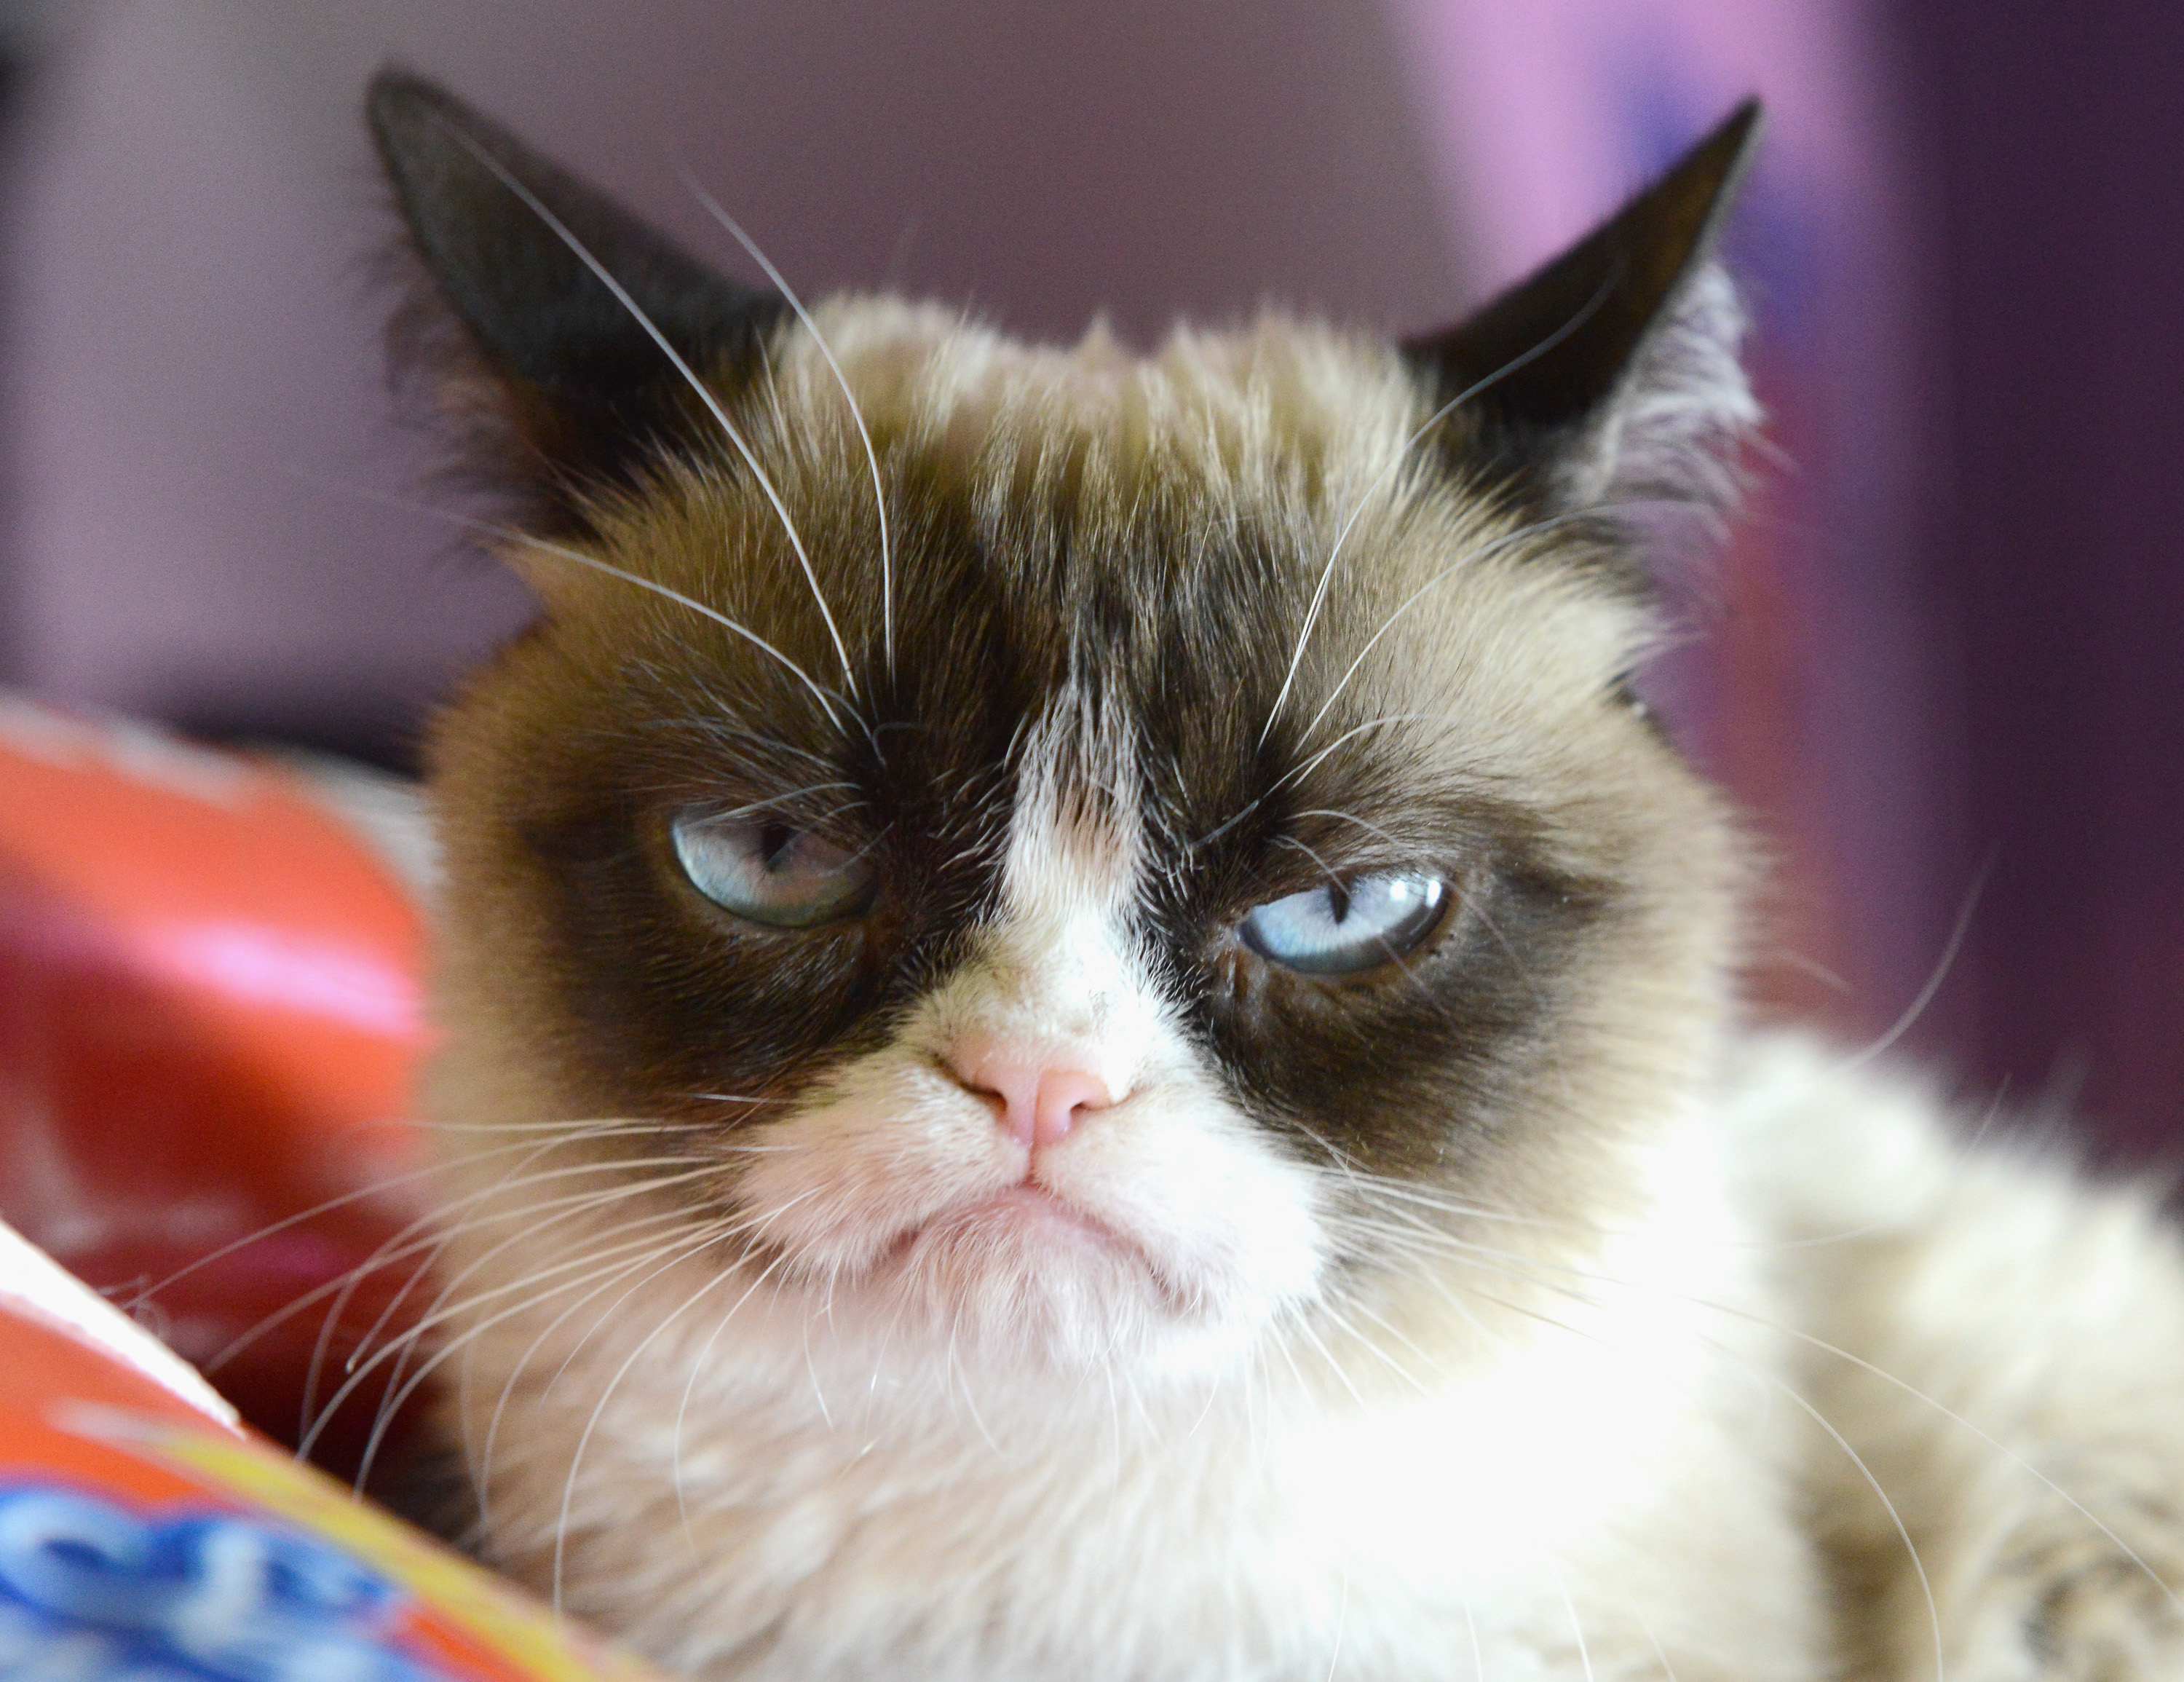
\includegraphics[width=0.75\linewidth]{image.jpg}|\\
\verb|	\caption{Dit is een voorbeeld van een figuur-float}|\\
\verb|	\label{fig:VoorbeeldFigFloat}|\\
\verb| \end{figure}|

 
 \begin{figure}[!ht]
 	\centering
 	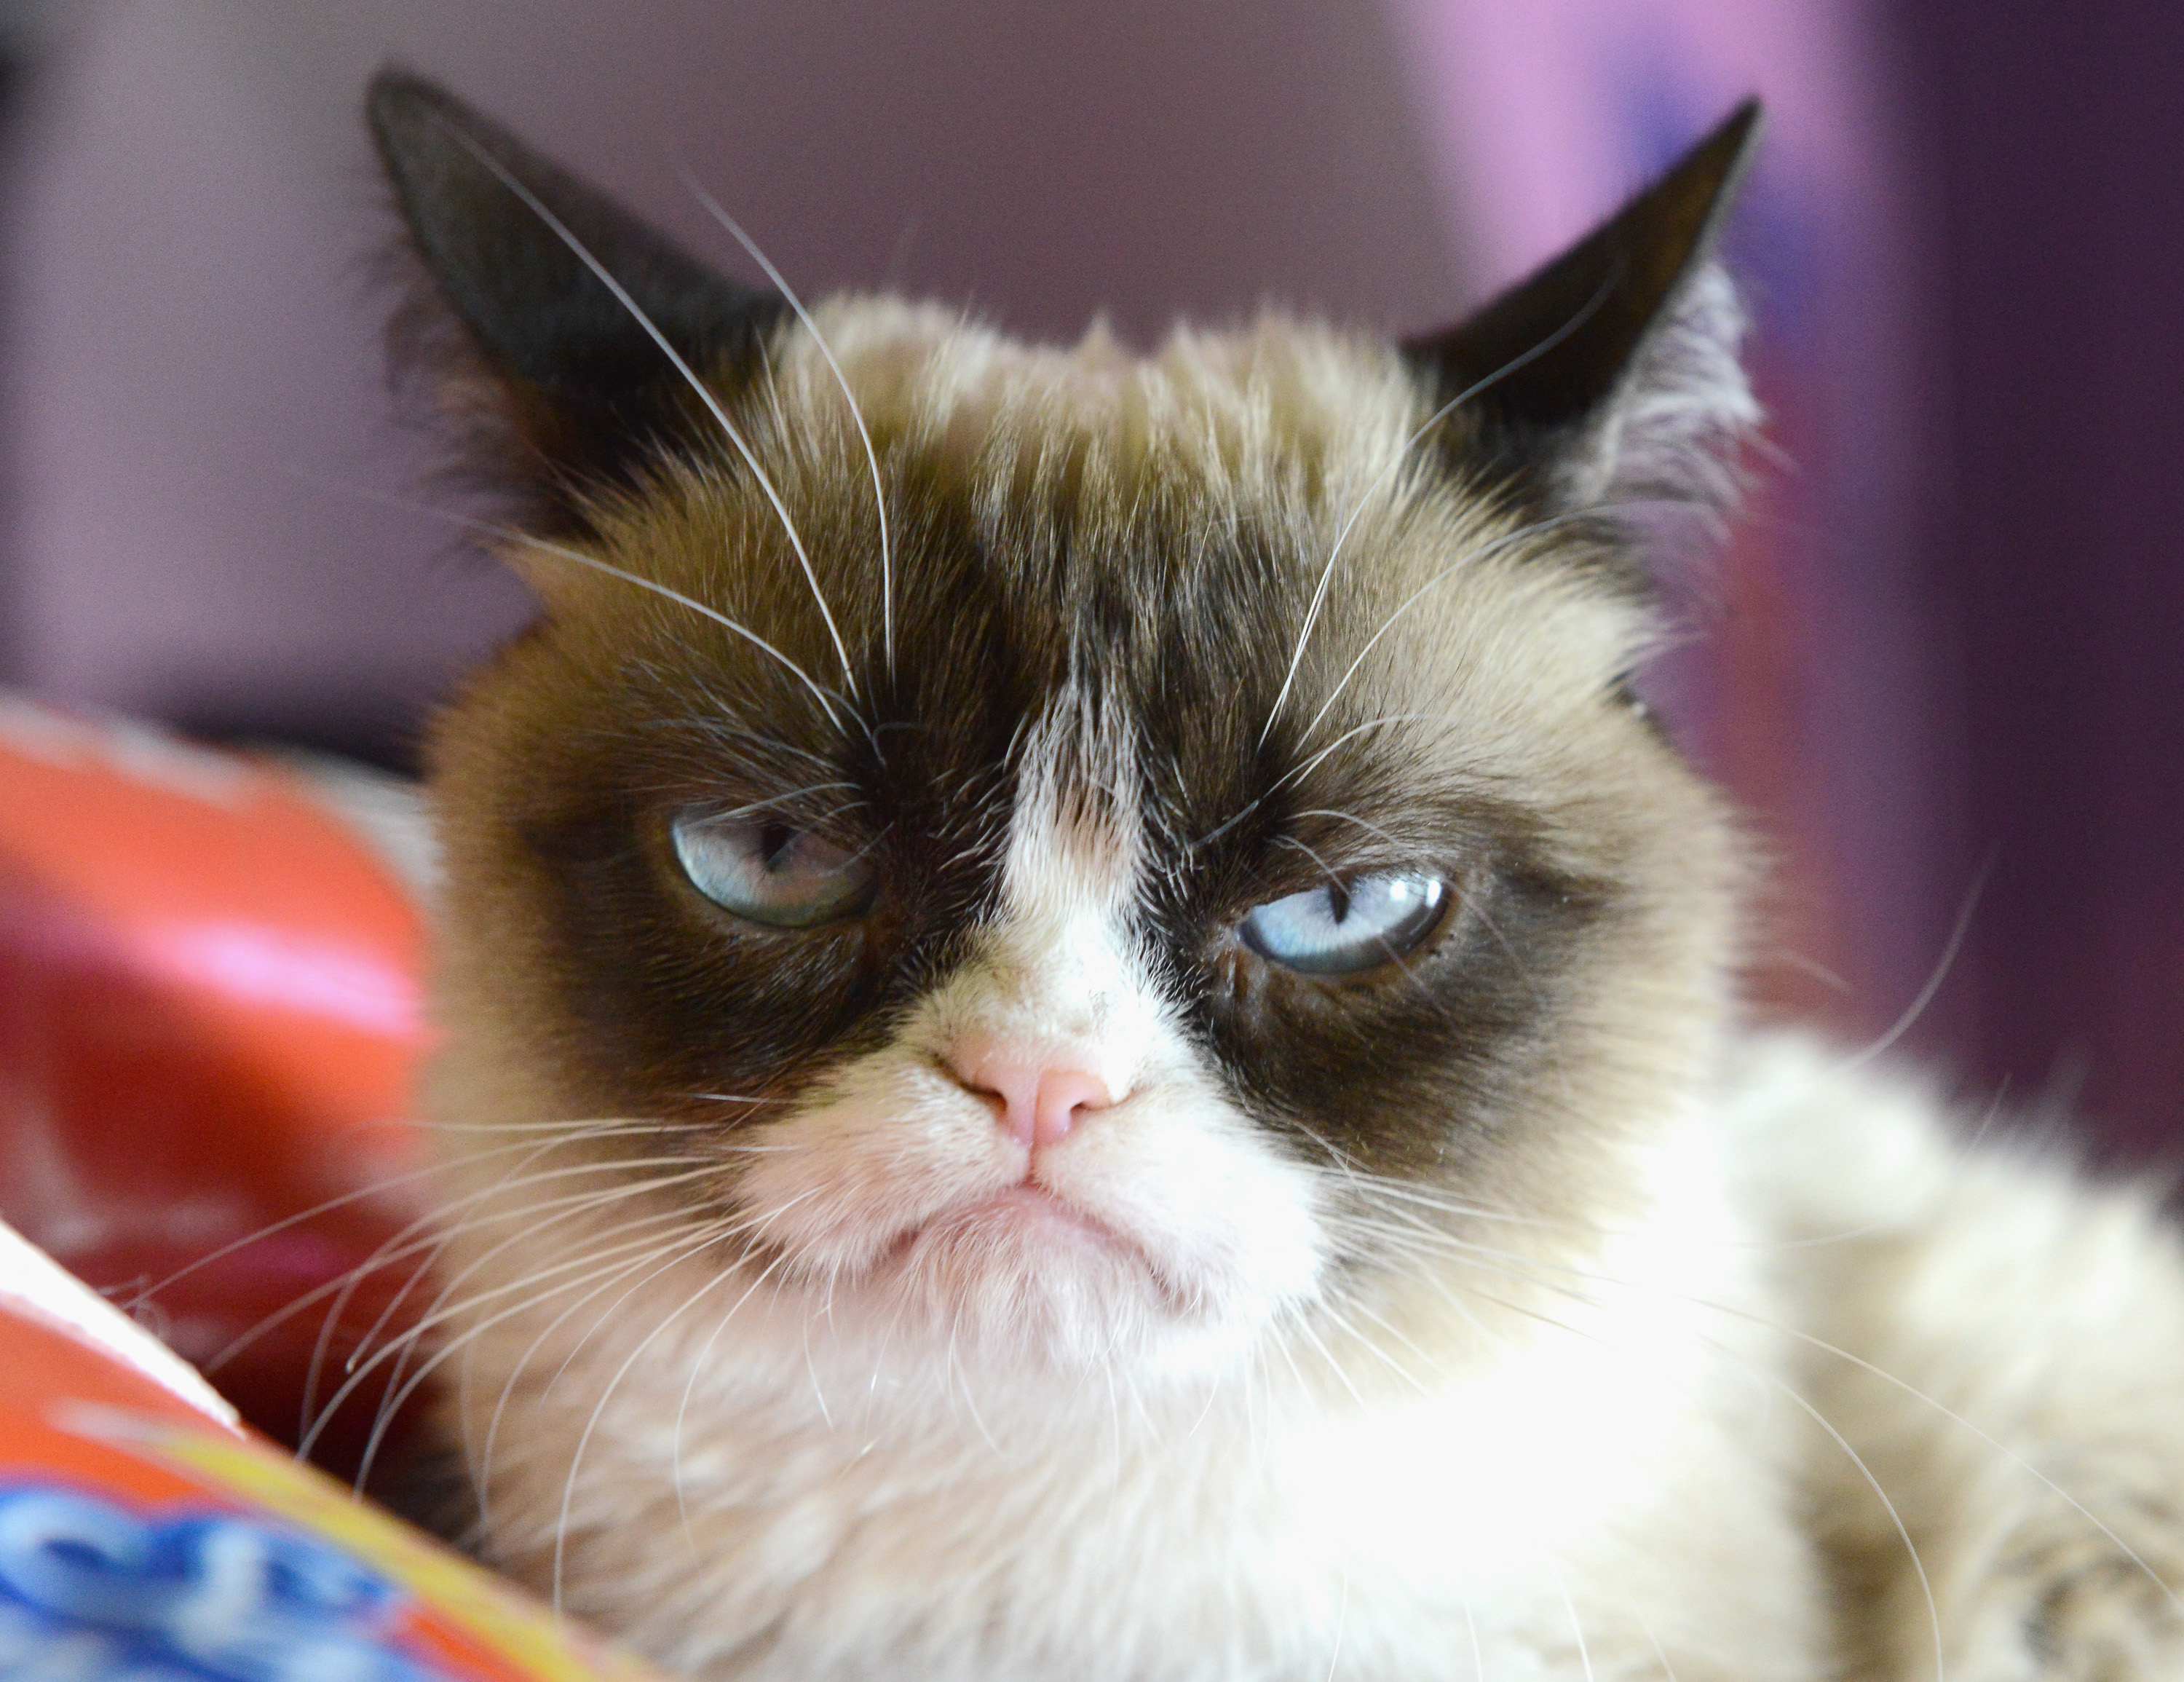
\includegraphics[width=0.75\linewidth]{image.jpg}
 	\caption{Dit is een voorbeeld van een figuur-float}
 	\label{fig:VoorbeeldFigFloat}
 \end{figure}

Tabellen worden links uitgelijnd op de bladzijde. Ook het bijschrift wordt links uitgelijnd en boven de tabel geplaatst. Na de tabelnummer volgt de beschrijving van de tabel. Tabel \ref{tab:VoorbeeldTableFloat} toont een voorbeeld van een eigen tabel. Vermijd om tabellen te kopie\"eren van andere werken, maar herwerk ze en plaats de nodige bronvermelding. De nodige syntax om tabel \ref{tab:VoorbeeldTableFloat} te generen wordt hieronder weergegeven:

\verb|\begin{table}[!ht]|\\
\verb|\caption{Dit is een voorbeeld van een tabel}|\\
\verb|\begin{tabular}{ccc}|\\
\verb|\hline|\\
\verb|Kolom 1 & Kolom 2 & Kolom 3\|\\
\verb|\hline|\\
\verb|1 & 2 & 3\\|\\
\verb|4 & 5 & 6\\|\\
\verb|\hline|\\
\verb|\end{tabular}|\\
\verb|\label{tab:VoorbeeldTableFloat}|\\
\verb|\end{table}|

Tot slot, let er op dat er expliciet naar elke tabel en figuur verwezen wordt vanuit de tekst. 

\begin{table}[!ht]
		\caption{Dit is een voorbeeld van een tabel}
	\begin{tabular}{ccc}
		\hline
		Kolom 1 & Kolom 2 & Kolom 3\\
		\hline
		1 & 2 & 3\\
		4 & 5 & 6\\
		\hline
	\end{tabular}
\label{tab:VoorbeeldTableFloat}
\end{table}
%%%%%%%%%%%%%%%%%%%%%%%%%%%%%%%%%%%%%%%%%%%%%%%%%%%%%%%%%%%%%%%%%%%% 
%                                                                 %
%                            CHAPTER                              %
%                                                                 %
%%%%%%%%%%%%%%%%%%%%%%%%%%%%%%%%%%%%%%%%%%%%%%%%%%%%%%%%%%%%%%%%%%% 
\chapter{Richtlijnen voor formules}

Er zijn twee manieren om formules in LaTeX in te voeren:

\begin{itemize}
	\item Inline: $a^2+b^2 = c^2$ (\verb|$a^2+b^2 = c^2$|)
	\item In een equation omgeving 	(\verb|\begin{equation}	a^2+b^2 = c^2	\end{equation}|):
	\begin{equation}
		a^2+b^2 = c^2
	\end{equation}

\end{itemize}

Griekse letters geef je in d.m.b. het backslash commando. Bijvoorbeeld de letter sigma $\sigma$ verkrijg je door \verb|$\sigma$| inline in te geven. Dit is analoog voor griekse letters in de equation omgeving. Een beknopte lijst van symbolen vind je op de Wikibooks pagina voor LaTeX (\href{https://nl.wikibooks.org/wiki/LaTeX/Wiskundige_formules}{link}). Alle andere nuttige informatie omtrent het gebruik van LaTeX voor formules vind je hier ook terug.
\cleardoublepage
%%%%%%%%%%%%%%%%%%%%%%%%%%%%%%%%%%%%%%%%%%%%%%%%%%%%%%%%%%%%%%%%%%%% 
%                                                                 %
%                            CHAPTER                              %
%                                                                 %
%%%%%%%%%%%%%%%%%%%%%%%%%%%%%%%%%%%%%%%%%%%%%%%%%%%%%%%%%%%%%%%%%%% 
\chapter{Richtlijnen voor referenties}

\section{Inleiding}
De referentielijst bevat de volledige lijst van literatuur en bronnen waarnaar in de tekst wordt verwezen. Door systematisch de referentielijst aan te vullen bij het schrijven van het literatuuroverzicht gaat er achteraf geen tijd verloren aan het opnieuw opzoeken van referenties.

\section{Referentiestijl}

Voor het verwijzen naar informatiebronnen wordt gebruik gemaakt van het numerisch systeem  of van het auteur-jaar systeem. Dit kies je door volgend commando in het latex bronbestand aan te passen:

\begin{itemize}
	\item numerisch (IEEE) : \verb|\bibliographystyle{ieee}|
	\item alfabetisch (APA) : \verb|\bibliographystyle{apalike}|
\end{itemize}

Plaats je bronnen in een \textit{bibtex} bestand (evt. via software zoals bv. Jabref Endnote of Mendeley), waarnaar je verwijst vanuit je thesis text a.d.h.v. het commando \verb|\cite|. Enkele links naar nuttige software in deze context:

\begin{itemize}
	\item \href{http://www.jabref.org/}{JabRef (Open Source)}
	\item \href{http://www.mendeley.com}{Mendeley (Freeware)}
	\item \href{http://www.endnote.com}{EndNote (Paid license)}
\end{itemize}

Indien je zelf een .bibtex bestand wil aanleggen dien je volgende syntax te volgen voor een tijdschriftartikel:
\clearpage
\verb|@article{hughes2005,|\\
\verb|title={Isogeometric analysis: CAD, finite elements, NURBS, exact geometry|\\ \verb|and mesh refinement},|\\
\verb|author={Hughes, Thomas JR and Cottrell, John A and Bazilevs, Yuri},|\\
\verb|journal={Computer methods in applied mechanics and engineering},|\\
\verb|volume={194},|\\
\verb|number={39},|\\
\verb|pages={4135--4195},|\\
\verb|year={2005},|\\
\verb|publisher={Elsevier}|\\
\verb|}|

Enkele voorbeelden van het gebruik van bronnen in een tekst (in APA stijl): 

Recent werd het Higgs boson experimenteel vastgesteld door Aad et al.\ \cite{aad2012} (syntax: \verb|\cite{aad2012}|). 

Als alternatief voor het discretiseren van een CAD model vooraleer een eindige elementenanalyse te kunnen toepassen, stellen Hughes et al.\ voor om de nodige elementenformulering rechtstreeks uit de NURBS beschrijving van de CAD geometrie te halen \cite{hughes2005} (syntax: \verb|\cite{hughes2005}|). Daarnaast introduceren ze tevens een k-iteratieve procedure als een verfijning van de geldende p- en h-iteratieve procedures in eindige elementen methoden \cite{cottrell2009} (syntax: \verb|\cite{cottrell2009}|).


%%%%%%%%%%%%%%%%%%%%%%%%%%%%%%%%%%%%%%%%%%%%%%%%%%%%%%%%%%%%%%%%%%% 
%                                                                 %
%                            CHAPTER                              %
%                                                                 %
%%%%%%%%%%%%%%%%%%%%%%%%%%%%%%%%%%%%%%%%%%%%%%%%%%%%%%%%%%%%%%%%%%% 

\chapter{Introduction}

blabla blabla tekst tekst.
%%%%%%%%%%%%%%%%%%%%%%%%%%%%%%%%%%%%%%%%%%%%%%%%%%%%%%%%%%%%%%%%%%% 
%                                                                 %
%                            CHAPTER                              %
%                                                                 %
%%%%%%%%%%%%%%%%%%%%%%%%%%%%%%%%%%%%%%%%%%%%%%%%%%%%%%%%%%%%%%%%%%% 

\chapter{Background information on DNA and DNA sequencing}
\label{ch:MBbackground}

\section{Biology and DNA}

\subsection{History of genetics and DNA}

\paragraph{Genetics}

\begin{wrapfigure}{R}{0.25\textwidth}
	%src: https://upload.wikimedia.org/wikipedia/commons/8/87/Gregor_Mendel_portrait.jpg
	\begin{center}
		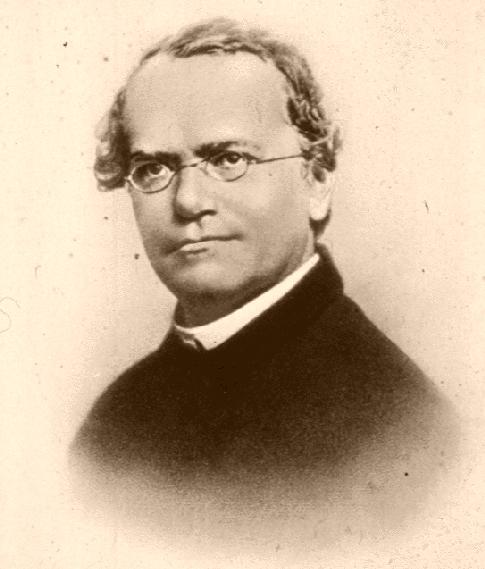
\includegraphics[width=0.20\textwidth]{background/GregorMendel.jpg}
		Gregor Mendel
	\end{center}
\end{wrapfigure}


For thousands of years, humans have observed the effects of heredity and implemented their knowledge to domesticate plants and animals. However, the science behind heredity was only started to be understood since 1859 with the publication of \emph{on the origin of species} by Charles Darwin. 

Around 1865, an Austrian monk and botanist Gregor Mendel, who studied at the university in Brno in the current Czech Republic, published his results on the hybridization studies of pea plants. He is often credited as being the father of modern genetics. In his findings, he implemented the role of \emph{factors} that influence the expression of traits. These factors later became known as \emph{genes}~\cite{Mendel}.

\paragraph{DNA}

In 1869, Swiss physician Friedrich Miescher discovered a microscopic substance in the pus of discarded surgical bandages. Later, in 1909, Phoebus Levene named this substance DeoxyriboNucleic Acid (DNA) since it is found in the nucleus of a cell and has acidic properties~\cite{Miescher}.

The full structure of DNA was discovered by Francis Crick and James Watson at the Cavendish Laboratory at the University of Cambridge~\cite{Crick}.

\subsection{Structure of DNA}

DNA, or Deoxyribonucleic Acid, is the molecule that stores the genetic information of all living organisms. It is the information that programs all of the activities in a cell.

Structurally, DNA is a polymer, which means each molecule is built up out of small repeating molecular units. In DNA, these units are called \emph{nucleotides}.

\begin{figure}[H]
	\centering
	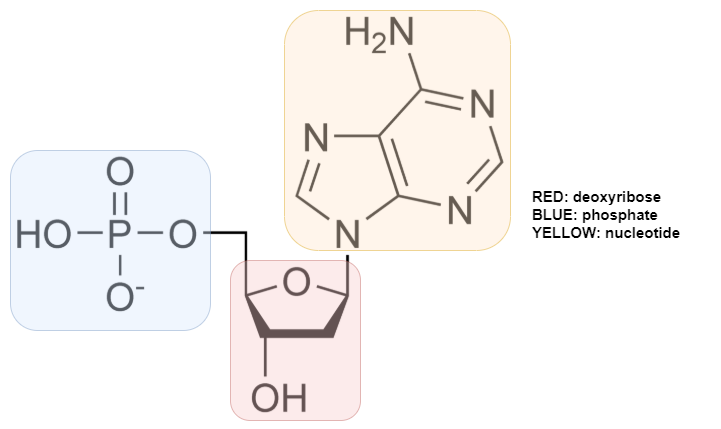
\includegraphics[width=0.75\linewidth]{background/Nucleotide.png}
	\caption{The structure of one nucleotide~\cite{Nucleotide}(modified from source).}
	\label{fig:nucleotide}
\end{figure}

Each nucleotide consists of 3 parts:

\begin{enumerate}
	\item A carbon sugar molecule called \emph{Deoxyribose}.
	\item A phosphate group to connect the Deoxyribose molecules. 
	\item One of four possible nitrogen bases: Adenine ($A$), Thymine ($T$), Cytosine ($C$) or Guanine ($G$).
\end{enumerate}

It is important to note that in most living organisms DNA does not exist as a single polymer, but rather a pair of molecules that are held tightly together. This is the famous \emph{double helix}.

\begin{figure}[H]
	%src: https://upload.wikimedia.org/wikipedia/commons/thumb/1/14/Double_stranded_DNA_with_coloured_bases.png/1024px-Double_stranded_DNA_with_coloured_bases.png
	\centering
	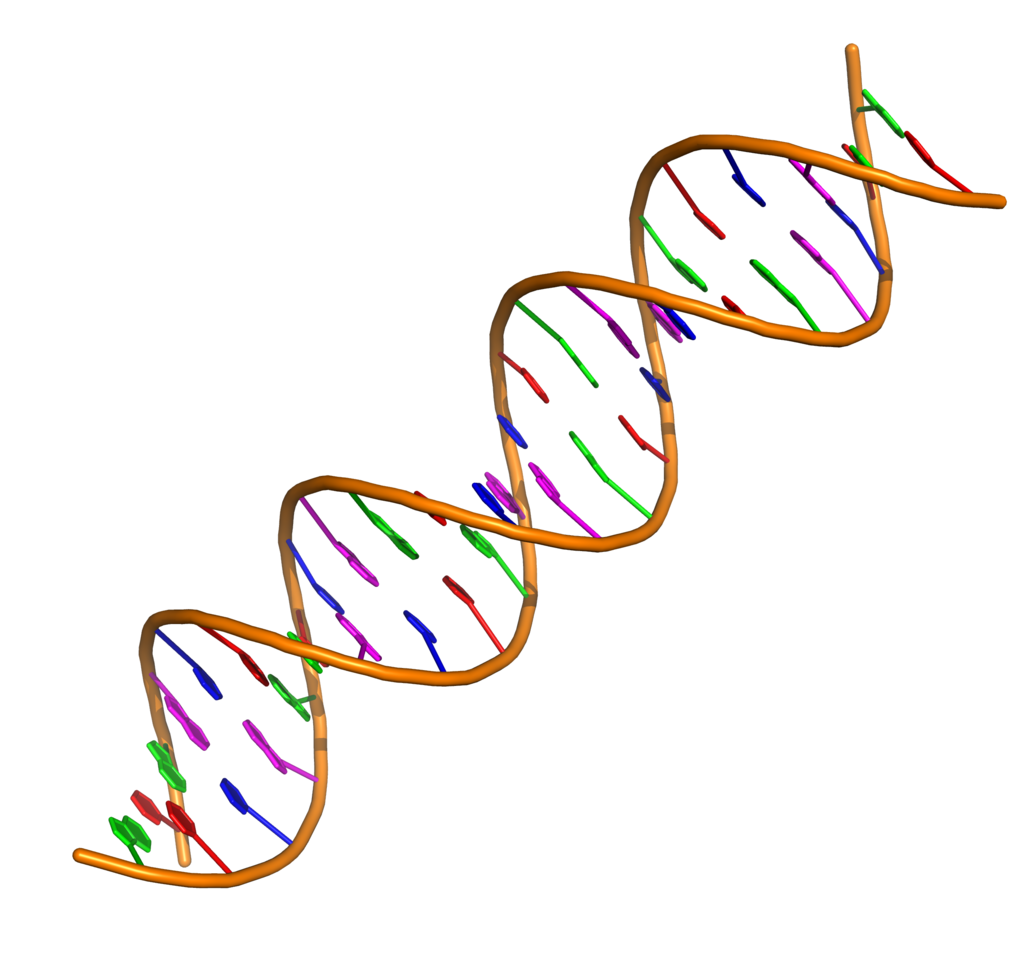
\includegraphics[width=0.3\linewidth]{background/DoubleHelix.png}
	\caption{The famous double helix~\cite{dna}.}
	\label{fig:doubleHelix}
\end{figure}

Like in any good structure, there is a need for the main support. In DNA, the sugars and phosphates bond together to form twin backbones. These sugar-phosphate bonds run down each side of the helix, but chemically in opposite directions. 

The first phosphate group, at the start of the molecule, connects to the sugar group's 5th carbon ($5'$). At the end of the structure, the 3rd carbon ($3'$) of the sugar group is unconnected. This makes a pattern typically noted as $[5' \rightarrow 3']$. Now, since the other molecule in the helix goes in the opposite direction, the pattern of the other backbone is typically noted as $[3' \rightarrow 5']$.

\begin{figure}[H]
	%src: https://upload.wikimedia.org/wikipedia/commons/thumb/e/e4/DNA_chemical_structure.svg/800px-DNA_chemical_structure.svg.png
	\centering
	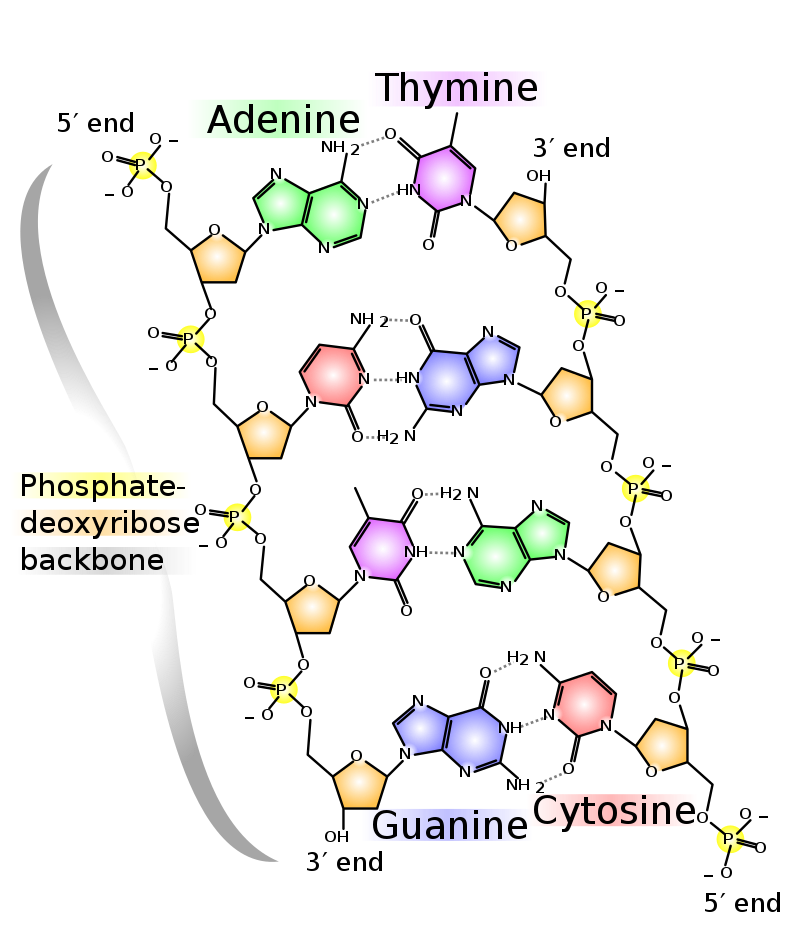
\includegraphics[width=0.5\linewidth]{background/DNAstructure.png}
	\caption{A short part of a DNA molecule containing a $[5' - ACTG - 3']$ (left) and a complementary strand of $[3' - TGAC - 5']$ (right). These 2 strands are interconnected by hydrogen bonds~\cite{dnachemical}.}
	\label{fig:DNAstructure}
\end{figure}

These two long chains are linked together by the nitrogen bases via their relatively weak hydrogen bonds, but there can't just be any pair of nitrogen bases. Adenine can only make hydrogen bonds with Thymine. Likewise, Guanine can only bond with Cytosine. These bonded nitrogen bases are called \emph{base paires}.

It is the order of these bases, which is also called the \emph{sequence}, that allows this DNA to store useful information. In this way, e.g. $AGGTCCATG$ means something completely different as a base sequence than e.g. $TTCCAGATC$.

Since each of the bases in the sequence has only one possible counterpart, you can predict what its matching counterpart will be in the opposite string. For example:

If the following sequence is known
$$[5' - AGGTCCG - 3']$$
we can deduce the sequence in the other direction as
$$[3' - TCCAGGC - 5']$$

//TODO einde zin = punt?

\subsection{DNA in the human body}

In human cells, DNA molecules can be found in the nucleus of all cells in the body. It consists of 46 very long molecules, which during cell division condense in what we call \emph{chromosomes}. The only exception is in reproductive cells (the egg cell and the sperm cell), which only have 23 chromosomes. 

The 23 chromosomes, which make up our whole DNA, are always present in pairs in the cells, making a total of 46 chromosomes. Each time, the pair consists of one chromosome from the father and the other one from the mother. 

The 23 chromosome pairs are classified in:
\begin{itemize}
	\item 22 pairs of autosomal chromosomes, marked 1 to 22 according to the length of the sequence. The longest chromosome (chromosome number-1) is 248,956,422 bases long. The shortest (chromosome number-22) is 50,818,468 bases long.
	\item In each cell, there is also an X chromosome plus an X or Y chromosome, dependent on the gender (XY for male, XX for female).
\end{itemize}


\begin{figure}[H]
	%src: https://upload.wikimedia.org/wikipedia/commons/thumb/b/b2/Karyotype.png/800px-Karyotype.png
	\centering
	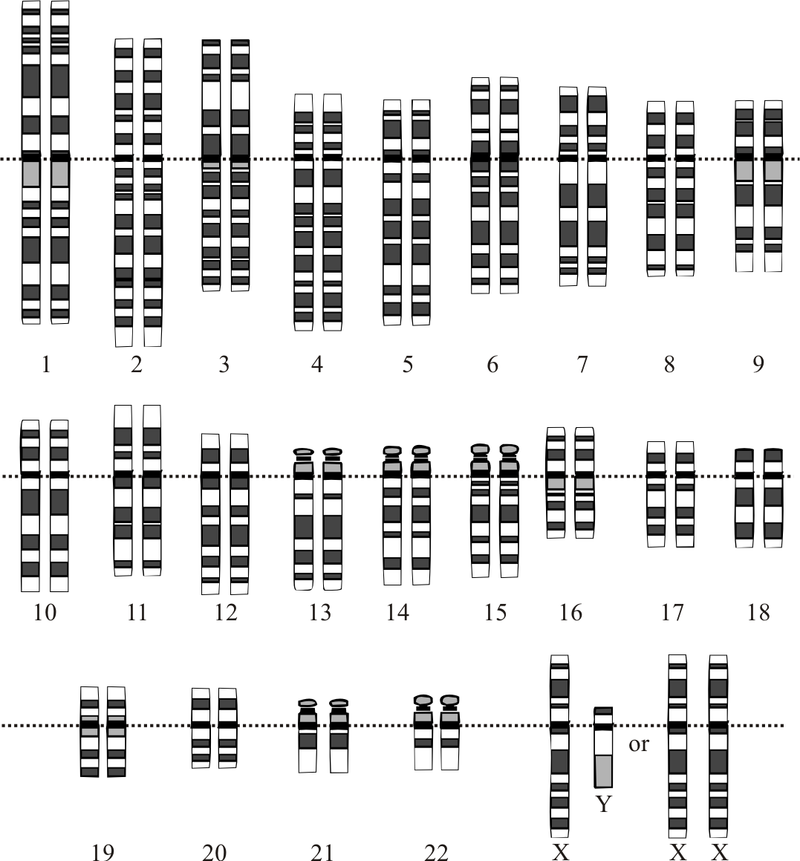
\includegraphics[width=0.5\linewidth]{background/karyotype.png}
	\caption{the 46 human chromosomes~\cite{8}.}
	\label{fig:karyotype}
\end{figure}

These chromosomes are packed tightly together in the nucleus of the cell. If all of these 46 chromosomes are put together, this makes about two times 3 billion base pairs. These 3 billion base pairs provide the assembly instructions for pretty much everything inside the cell.


\section{The Human Genome Project}

In the field of Bioinformatics, an important dataset is the \emph{Human Genome}. This is the full DNA sequence found in the Nucleus, ordered from chromosome 1 to 22, followed by the X and Y chromosome.

In October 1990, biologists in the relatively new field of molecular biology started the Human Genome Project. The goal of this project was to determine the sequence of the 3 billion base pairs that make up human DNA. This project was completed and published in 2003. So, nowadays we have a good idea of how the human genome is built up.

The Human Genome is easily found on the internet since it is publically available. One of the most often used assembly is \emph{hg19}, which was published in 2009. Since DNA has only 4 possible bases ($A$, $T$, $C$ or $G$), this can be encoded in a 2-bit representation. If this encoding is used, ideally the Human Genome is approximately 750 megabytes.

\begin{figure}[H]
	\centering
	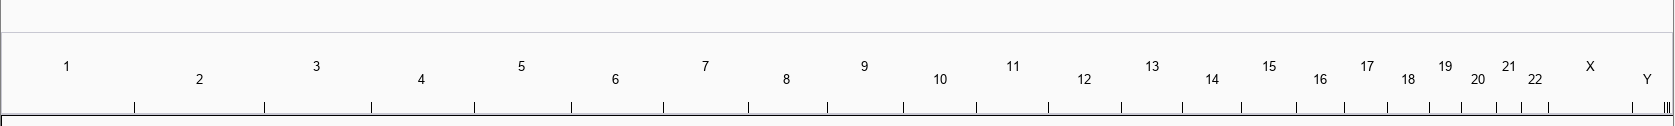
\includegraphics[width=\linewidth]{background/HG.png}
	\caption{The order and the sizes of the chromosomes of the human genome as depicted in the IGV software~\cite{IGV}.}
	\label{fig:HG}
\end{figure}

\section{Sequencing}

\subsection{The sequencing technology}

The term \emph{Sequencing} is used for all techniques to read and decipher the DNA code from a given snippet of DNA. During the last years, the techniques that sequence human DNA has changed quite a lot. For about 15 years the \emph{Next Generation Sequencing (NGS)} is the technique most often used. The biggest advantage of NGS, in comparison with other techniques, is the speed of the sequencing since it can sequence billions of short DNA molecules in parallel. In practice, this sequencing is most often done by the instruments of the company Illumina, which dominates the market (around 90\% market share).

\paragraph{How whole-genome NGS works}

\begin{enumerate}
	\item The DNA to sequence is isolated from the cells. Most often this is the whole genome.
	\item  In some cases, the isolated DNA can now be copied enzymatically. This step is repeated until there are enough copies of the same DNA. Usually, this is in the millions or billions of copies.
	
	\begin{figure}[H]
		%src: file:///D:/Erasmus/thesis/interessante%20papers/masterthesis%20BFAST%20op%20FPGA.pdf
		\centering
		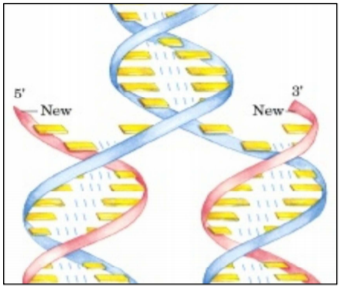
\includegraphics[width=0.3\linewidth]{background/enzymCopying.png}
		\caption{The enzymatic copying of a string of DNA. The original is unzipped, thus allowing new nucleotide bases to attach to the exposed bases~\cite{}.}
		\label{fig:enzymCopying}
	\end{figure}
	
	\item The full DNA sequence is now broken apart into small DNA molecules (100 to 1000 bases long). This is done using enzymes or high-frequency sound waves.
	\item Now the sequencing can start: a \emph{flow cell} is used where these small DNA molecules can bind to a glass surface. 
	\item Different enzymatic and chemical reactions can now be done on this flow cell through an automatic flow of reagents. The following steps are iterated until the full read has been filled in:
	\begin{enumerate}
		\item The entire flowcell is filled with nucleotides, all with different nitrogen bases. Important is that at each of these nucleotides there is a fluorescent group attached. This also makes sure no other nucleotide can bind.
		\item The fluorescent groups have a different color, dependent on the nitrogen base attached ($A$, $G$, $T$ of $C$). At this time a camera picture of the flowcell is taken and stored.
		\item After the flowcell is emptied of the loose nucleotides, another reagent flows in this flowcell. This reagent splits the fluorescent group so that in the next iteration a new nucleotide group can bind with the read.
		
		\begin{figure}[H]
			%src: file:///D:/Erasmus/thesis/interessante%20papers/masterthesis%20BFAST%20op%20FPGA.pdf
			\centering
			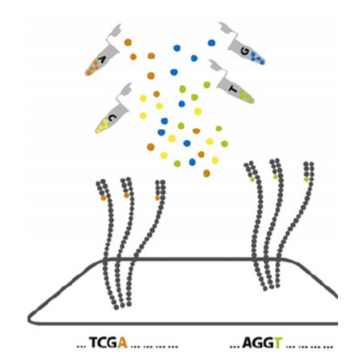
\includegraphics[width=0.5\linewidth]{background/NGS.png}
			\caption{Sequencing technology used by Illumina attaches a nucleotide with a fluorescent tag to the next base in the read, then it captures a picture to determine the base, and removes the fluorescent tag so a new nucleotide group can bind in the next iteration~\cite{}.}
			\label{fig:NGS}
		\end{figure}
	\end{enumerate}
	
	\item After the whole DNA snippets have been filled in, the machine deduces the sequence in the DNA snippet. The pictures that were taken in order during the operation show the colors released in a specific spot, and by extent the attached nitrogen base. By the means of some image processing techniques, it is quite easy to get all the sequences from all the molecules bound on the flowcell. This is called the \emph{Primary processing}.
	
	\begin{figure}[H]
		%src: PPT van Howest
		\centering
		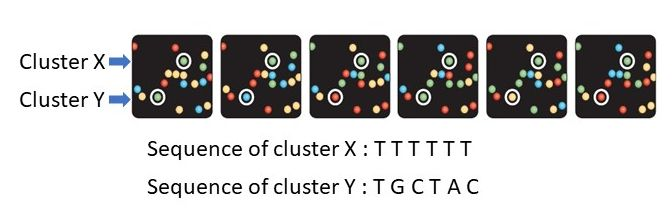
\includegraphics[width=\linewidth]{background/ImProc.jpg}
		\caption{From left to right are the pictures taken at each iteration in the flowcell. The color at that specific spot marks which nucleotide has been bound. With the use of some image processing techniques the exact sequence in that spot can be identified~\cite{pptHowest}.}
		\label{fig:ImProc}
	\end{figure}
	
	\item In the \emph{secundary processing}, the sequence is trimmed by quality, etc. The operations that are done on the read in this step are outside the scope of this thesis.
\end{enumerate}

As a result of the NGS, we get a (large) file in the FASTQ format.

\subsection{The FASTQ file format}
\label{expl:FASTQ}

Since the color of each spot observed in the camera pictures in the primary processing can have a light shift, there is a specific "uncertainty" about the correct base is in that spot. This is called the \emph{quality} of the base.

The \emph{FASTQ} file format has become the de-facto standard as output from sequencing instruments. It is a text-based format for storing both the bases in the sequence and their corresponding quality.

A FASTQ file uses four lines per sequenced DNA fragment:

\begin{enumerate}
	\item A '$@$' character followed by a sequence ID, plus an optional description. This description mostly contains the coordinate of the spot on the flowcell.
	\item \label{enumIt:fastqRaw} The sequence of DNA bases identified by the machine. This is either $A$, $G$, $C$, $T$, or $n$ when the base cannot be identified with a specific threshold certainty.
	\item A '$+$' character, optionally followed by the sequence ID (again) and an optional description.
	\item The quality values for each respective base in line~\ref{enumIt:fastqRaw}. The length of this line must be the same as the number of bases in line~\ref{enumIt:fastqRaw}.
\end{enumerate}

The quality score in memory is a value in the range $0x21$ (lowest quality) to $0x7e$ (highest quality). Since this value is represented in ASCII in the file format, this ranges from the '$!$' character to the '$\mathtt{\sim}$' character. Hereunder is a complete list of the possible values of the quality score:

\begin{lcverbatim}
!"#$%&'()*+,-./0123456789:;<=>?@ABCDEFGHIJKLMNOPQRSTUVWXYZ
[\]^_`abcdefghijklmnopqrstuvwxyz{|}~
\end{lcverbatim}


Important to note is that this quality score is logarithmic. Also, the '$@$' and '$+$' character are a possible value for the quality, so this will be something to look out for when implementing the interpreter for this file.\\

	
A FASTQ file containing a single sequence of a DNA fragment of 55 bases might look like this:


\begin{lcverbatim}
@P3018:1114
GCTACTTCCCAAGAAGCTGTTCAGAATCAGAATGAGCCGCAACTTCGGGATGAAA
+
AAAAAEEEEEEEEEEEEEEEEEEEEEEFFFFFFGGGGGIIIJJKKKKLLLLLMMM
\end{lcverbatim}

Keep in mind that a FASTQ file consists of multiple of these sequences, all stacked under each other.
	
	

%%%%%%%%%%%%%%%%%%%%%%%%%%%%%%%%%%%%%%%%%%%%%%%%%%%%%%%%%%%%%%%%%%% 
%                                                                 %
%                            CHAPTER                              %
%                                                                 %
%%%%%%%%%%%%%%%%%%%%%%%%%%%%%%%%%%%%%%%%%%%%%%%%%%%%%%%%%%%%%%%%%%% 

\chapter{Platforms for sequence alignment algorithms}

Most sequence alignment algorithms are heavily parallelisable. An overview of the most frequently used algorithms is given in chapter \ref{ch:algoverzicht}.

\section{Overview of possible hardware}

\section{CPU}
\section{GPU}
\section{FPGA}
\section{ASIC}



%%%%%%%%%%%%%%%%%%%%%%%%%%%%%%%%%%%%%%%%%%%%%%%%%%%%%%%%%%%%%%%%%%% 
%                                                                 %
%                            CHAPTER                              %
%                                                                 %
%%%%%%%%%%%%%%%%%%%%%%%%%%%%%%%%%%%%%%%%%%%%%%%%%%%%%%%%%%%%%%%%%%% 

\chapter{Methods for genetic sequence alignment}
\label{ch:algoverzicht}


\section{Genetic sequence aligning}

The human genome (e.g. $HG19$) is used as a reference genome for all sequenced human DNA. However, The genetic code of all humans is slightly different. Genetic sequence alignment is the science where you try to align 2 sequences with each other so that the amount of differences is minimal. In this chapter, the most frequently used algorithms are examined.

\subsection{Alignment in general}

In genetic codes, there are 3 types of differences between the given sequence and the reference:

\begin{itemize}
	\item Insertion: one or more bases have been added in the genetic code in a specific spot.
	\item Deletion: one or more bases have been removed from the genetic code in a specific spot.
	\item Substitution: one or more bases have been substituted by other bases.
\end{itemize}

Inserts and deletions are often described by a single term, \emph{indel}. In literature, this is most often represented with a '$-$' character.\\

For example: if we want to align the following sequences:
\begin{lcverbatim}
	Seq1: ATATCGGC
	Seq2: ATCG
\end{lcverbatim}
The alignment itself can now be done in different ways. Possible alignments are:
\begin{lcverbatim}
	Alignment 1
	Seq1: AtaTCgGc
	Seq2: A--TC-G-
	Alignment 2
	Seq1: atATCGgc
	Seq2: --ATCG--
\end{lcverbatim}
Which alignment that is the actual output, depends on the algorithm and the given parameters.

Keep in mind, there is no one "correct" alignment. The core of the alignment algorithms is the same each time, but the parameters of these algorithms are changed depending on the application.

\section{Local VS global alignment}



\section{commonly used algorithms}

\subsection{Dynamic programming algorithms}
\subsubsection{Needleman-Wunsch}
\subsubsection{Smith-Waterman}

\subsection{Heuristic algorithms}
\subsubsection{FASTA}
\subsubsection{BLAST}

\section{Problem definition and algorithm selection}

\subsection{Mapping to a reference genome}

\subsection{Clinical application}
%%%%%%%%%%%%%%%%%%%%%%%%%%%%%%%%%%%%%%%%%%%%%%%%%%%%%%%%%%%%%%%%%%% 
%                                                                 %
%                            CHAPTER                              %
%                                                                 %
%%%%%%%%%%%%%%%%%%%%%%%%%%%%%%%%%%%%%%%%%%%%%%%%%%%%%%%%%%%%%%%%%%% 

\chapter{Initial approach with pure Smith-Waterman}

\section{The concept}

\section{System implementation}

\section{Possible initial speedups}

\section{Problems with this initial approach}

computational complexity: O(mn)


%%%%%%%%%%%%%%%%%%%%%%%%%%%%%%%%%%%%%%%%%%%%%%%%%%%%%%%%%%%%%%%%%%% 
%                                                                 %
%                            CHAPTER                              %
%                                                                 %
%%%%%%%%%%%%%%%%%%%%%%%%%%%%%%%%%%%%%%%%%%%%%%%%%%%%%%%%%%%%%%%%%%% 

\chapter{Acccelerating the software implementation using HLS}

\section{Analysing software performance}

In the SDSoC environment, it is possible to analyse the software running on the SoC chip using a TCF profiler. After running this analysis, the TCF profiler returns an overview of the functions, sorted on the amount of time spent when running. The analysis is shown in figure \ref{fig:softwareFunctionUsage}

\begin{figure}[H]
	\centering
	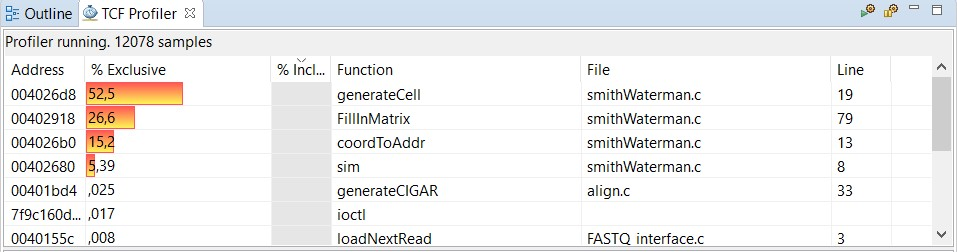
\includegraphics[width=0.75\textwidth]{speedup/softwareFunctionUsage.jpg}
	\caption{a TCF profile of the software implementation}
	\label{fig:softwareFunctionUsage}
\end{figure}

When examining this analysis, we should keep in mind that the generateCell, coordToAddr and sim functions are inline functions used in the FillInMatrix method. Just as suspected the software spends almost all of its time in these methods, so it's worth it to try to accelerate these functions.

\section{Recoding parts of the software to be more hardware friendly}

Back in 2011, Vermij E. did a thesis on RVE (recursive variable expansion). In it, he discusses the most efficient ways to program a processing element to generate one value in the alignment matrix. His results can be found in figure \ref{fig:PE}. 

\begin{figure}[H]
	%src=file:///D:/Erasmus/thesis/interessante%20papers/masterthesis%20Smith-Waterman%20op%20FPGA%20(TU%20Delft).pdf
	\centering
	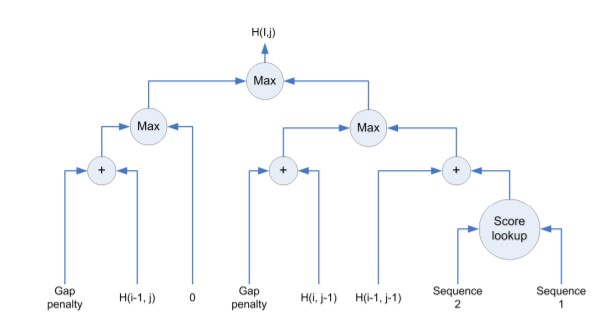
\includegraphics[width=0.75\textwidth]{speedup/PE.jpg}
	\caption{The optimal processing found in the thesis from Vermij E.}
	\label{fig:PE}
\end{figure}

It seemed like a good idea to reimplement the generatecell function, using this newly found scheme. However, it is also important to keep track of where the value comes from. Therefore, the following (new) code was adopted for generating a cell:

\begin{lcverbatim}
//calculate the possible  values
CELL diagonalCELL = { diagonal.value + sim(refVal, seqVal), 1 };
CELL leftCELL = { left.value - gp, 2 };
CELL upCELL = { up.value - gp, 3 };
CELL zeroCELL = { 0, 0 };

CELL upstreamA = (leftCELL.value > upCELL.value) ? leftCELL : upCELL;
CELL upstreamB = (diagonalCELL.value > zeroCELL.value) ? 
					diagonalCELL : zeroCELL;

CELL newCell = (upstreamA.value > upstreamB.value) ? upstreamA : upstreamB;

//Return the cell:
return newCell;
\end{lcverbatim}

Where the second attribute in the CELL type is the direction.

\section{Hardware acceleration}

It turns out, HLS does not support in/out matrix to memory yet.

slices

direction of matrix (first column then row).

Bitwidth of (packed) data on axi master must be power of 2. => change the int to int16\_t and direction to uint16\_t (really wastefull towards memory) but no other choice without major remodel.

\section{Comparison with the software}
%%%%%%%%%%%%%%%%%%%%%%%%%%%%%%%%%%%%%%%%%%%%%%%%%%%%%%%%%%%%%%%%%%% 
%                                                                 %
%                            CHAPTER                              %
%                                                                 %
%%%%%%%%%%%%%%%%%%%%%%%%%%%%%%%%%%%%%%%%%%%%%%%%%%%%%%%%%%%%%%%%%%% 

\chapter{implementation results and speedup}

...
%%%%%%%%%%%%%%%%%%%%%%%%%%%%%%%%%%%%%%%%%%%%%%%%%%%%%%%%%%%%%%%%%%% 
%                                                                 %
%                            CHAPTER                              %
%                                                                 %
%%%%%%%%%%%%%%%%%%%%%%%%%%%%%%%%%%%%%%%%%%%%%%%%%%%%%%%%%%%%%%%%%%% 

\chapter{Conclusion and future research}

Gap opening and extension

BFAST algorithm

BASE type memory efficient

FTP for easy on and offloading the data

SEQ\_INDEX type maken memory efficient (75-300)


% Bibliografie: referenties. De items zitten in bibliografie.bib
%%%%%%%%%%%%%%%%%%%%%%%%%%%%%%%%%%%%%%%%%%%%%%%%%%%%%%%%%%%%%%%%%
% Indien je ook de niet geciteerde werken in je bibliografie wil opnemen, commentarieer dan onderstaande regel uit!
%\nocite{*}
\bibliographystyle{apalike}
\bibliography{bibliografie}

% Eventueel enkele appendices
%%%%%%%%%%%%%%%%%%%%%%%%%%%%%%
\appendix
\chapter{Implementation code}

The implementation code can also be found on Github: \href{https://github.com/robinno/refGenMapping}{https://github.com/robinno/refGenMapping}

\section{Filesystem organization}

To keep the code manageable, it was split up in multiple files. These files were organized in the directory structure as seen in figure \ref{fig:dirStruct}

\begin{figure}[H]
	\centering
	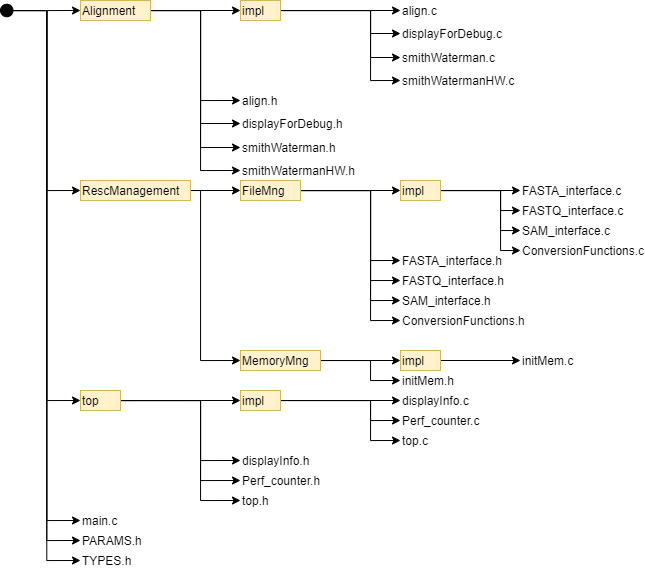
\includegraphics[width=0.8\textwidth]{code/dirStructure.png}
	\caption{The used directory structure in the implementation. Directories are colored in yellow.}
	\label{fig:dirStruct}
\end{figure}

\section{Code}
%listing all code files

{\setstretch{1.0} %interlinie afstand
	
\textbf{PARAMS.h}
\lstinputlisting[language=C]{sourceCode/PARAMS.h}
\textbf{TYPES.h}
\lstinputlisting[language=C]{sourceCode/TYPES.h}
\textbf{main.c}
\lstinputlisting[language=C]{sourceCode/main.c}


\textbf{top.h}
\lstinputlisting[language=C]{sourceCode/top/top.h}
\textbf{top.c}
\lstinputlisting[language=C]{sourceCode/top/impl/top.c}
\textbf{displayInfo.h}
\lstinputlisting[language=C]{sourceCode/top/displayInfo.h}
\textbf{displayInfo.c}
\lstinputlisting[language=C]{sourceCode/top/impl/displayInfo.c}
\textbf{Perf\_counter.h}
\lstinputlisting[language=C]{sourceCode/top/Perf_counter.h}
\textbf{Perf\_counter.c}
\lstinputlisting[language=C]{sourceCode/top/impl/Perf_counter.c}


\textbf{ConversionFunctions.h}
\lstinputlisting[language=C]{sourceCode/RescManagement/FileMng/ConversionFunctions.h}
\textbf{ConversionFunctions.c}
\lstinputlisting[language=C]{sourceCode/RescManagement/FileMng/impl/ConversionFunctions.c}
\textbf{FASTA\_interface.h}
\lstinputlisting[language=C]{sourceCode/RescManagement/FileMng/FASTA_interface.h}
\textbf{FASTA\_interface.c}
\lstinputlisting[language=C]{sourceCode/RescManagement/FileMng/impl/FASTA_interface.c}
\textbf{FASTQ\_interface.h}
\lstinputlisting[language=C]{sourceCode/RescManagement/FileMng/FASTQ_interface.h}
\textbf{FASTQ\_interface.c}
\lstinputlisting[language=C]{sourceCode/RescManagement/FileMng/impl/FASTQ_interface.c}
\textbf{SAM\_interface.h}
\lstinputlisting[language=C]{sourceCode/RescManagement/FileMng/SAM_interface.h}
\textbf{SAM\_interface.c}
\lstinputlisting[language=C]{sourceCode/RescManagement/FileMng/impl/SAM_interface.c}


\textbf{initMem.h}
\lstinputlisting[language=C]{sourceCode/RescManagement/MemoryMng/initMem.h}
\textbf{initMem.c}
\lstinputlisting[language=C]{sourceCode/RescManagement/MemoryMng/impl/initMem.c}


\textbf{align.h}
\lstinputlisting[language=C]{sourceCode/Alignment/align.h}
\textbf{align.c}
\lstinputlisting[language=C]{sourceCode/Alignment/impl/align.c}
\textbf{displayForDebug.h}
\lstinputlisting[language=C]{sourceCode/Alignment/displayForDebug.h}
\textbf{displayForDebug.c}
\lstinputlisting[language=C]{sourceCode/Alignment/impl/displayForDebug.c}
\textbf{smithWaterman.h}
\lstinputlisting[language=C]{sourceCode/Alignment/smithWaterman.h}
\textbf{smithWaterman.c}
\lstinputlisting[language=C]{sourceCode/Alignment/impl/smithWaterman.c}
\textbf{smithWatermanHW.h}
\lstinputlisting[language=C]{sourceCode/Alignment/smithWatermanHW.h}
\textbf{smithWatermanHW.c}
\lstinputlisting[language=C]{sourceCode/Alignment/impl/smithWatermanHW.c}
} %end line stretch




% Back cover: change according to the correct campus
% 
\includepdf{private/back_fiiw_denayer.pdf}
% 
\includepdf{private/back_fiiw_denayer_eng.pdf} % For the english version
%
\includepdf{private/back_fiiw_geel.pdf}
% 
\includepdf{private/back_fiiw_geel_eng.pdf} % For the english version
%
\includepdf{private/back_fiiw_gent.pdf}
% 
\includepdf{private/back_fiiw_ghent_eng.pdf} % For the english version

\includepdf{private/back_fiiw_brugge.pdf}
% 
\includepdf{private/back_fiiw_bruges_eng.pdf} % For the english version
%
\includepdf{private/back_fiiw_groept.pdf}
% \includepdf{private/back_fiiw_groupt_eng.pdf} % For the english version

\end{document}
